\documentclass[../../main.tex]{subfiles}
\begin{document}

\subsection*{8.2}
Due fili indefiniti distanti 2a=4cm, paralleli all'asse x solo percorsi indicati in figura.
\\Calcolare il campo magnetico $\vec{B}(z)$ sull'asse dei due fili e a quale distanza dal centro O si arresti un piccolo magnete lanciato con velocità $v_0 = 7.1 * 10^{-2}\frac{m}{s}$ da O lungo l'asse z, di massa $mg = 3.97 * 10^{-2}kg$ e momento magnetico $m=0.2Am^2$ parallelo e concorde a B.
\\Si assume che l'asse z orizzontale.
\\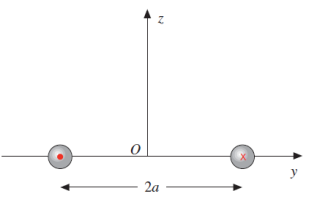
\includegraphics[scale=0.3]{e_8_2_0.png}
\\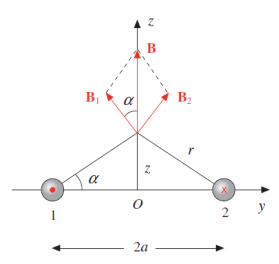
\includegraphics[scale=0.3]{e_8_2_1.png}
\subsubsection*{Formule utilizzate}
\subsubsection*{Soluzione punto a}
$\vec{B} = \frac{\mu_oi\vec{u_\phi}}{2\pi r}$ con $r = \sqrt{a^2+z^2}$   $\alpha=\frac{a}{r}$
\\$B_{1z} = B_1\cos\alpha$   $B_{1y}=-B_1\sin\alpha$
\\$B_{2z} = B_2\cos\alpha$   $B_{2y}=B_2\sin\alpha$
\\$B_z = B_{1z} + B_{2z}$   $B_y = 0$
\subsubsection*{Soluzione punto b}
$\Delta U = U(f)-U(i) = -mB_f + mB_i$
\\con $v_i =v_0$   $v_f = 0$
\\$\Delta E_c = -\Delta U_p$
\\$E_c(0) + U_p(0) = E_c(z) + U_p(z)$
\\$E_c(z) = 0$   $U_p = -mB$
\\$B(0) = \frac{\mu_0ia}{\pi a^2} = \frac{\mu_0 i}{\pi a}$
\newpage

\end{document}